\documentclass{article}
%packages
\usepackage{graphicx}
\usepackage[utf8]{inputenc}
\usepackage[T1]{fontenc}
\usepackage[frenchb]{babel}
\usepackage[a4paper]{geometry}
\usepackage{minted}
\usepackage{hyperref}
\usepackage{textcomp}

\begin{document}
%title
\begin{titlepage}
	\vspace{-20px}
	\begin{tabular}{l}
		\textsc{Blin} Sébastien\\
		\textsc{Collin} Pierre-Henri
	\end{tabular}
	\hfill \vspace{10px}
\includegraphics[scale=0.1]{../../../esir.png}\\
	\vfill
	\begin{center}
		\Huge{École supérieure d'ingénieurs de Rennes}\\
		\vspace{1cm}
		\LARGE{2ème Année}\\
		\large{Parcours Informatique}\\
		\vspace{0.5cm}\hrule\vspace{0.5cm}
		\LARGE{\textbf{Architecture Logicielle}}\\
		\Large{Compte-Rendu TP n\textdegree 1}
		\vspace{0.5cm}\hrule
		\vfill
		\vfill
	\end{center}
	\begin{flushleft}
		\Large{Sous l'encadrement de~:}\\
		\vspace{0.2cm}
		\large{\textsc{Temple} Paul}
	\end{flushleft}
	\vfill
\end{titlepage}

\section{Descriptif du projet}
Permettre d'avoir tout un processus de compilation (de la gestion de dépendance/installation du projet en local/tests/relecture du code (QA) par un tiers/vérification des builds sur toutes les plateformes/paramétrer les releases des versions.)
\section{Maven}
\subsection{Description}
\subsection{Utilisation}
\subsubsection{Génération de projets}
\subsubsection{Génération de rapports}
\subsubsection{Génération de packages}
\subsubsection{Tests}
\subsection{Pourquoi l'utiliser ?}


\section{SonarQube}
\subsection{Description}
SonarQube est une plateforme open-source utilisée en QA. Cet outil sert à vérifier (analyse statique) les règles de mise en forme, la complexité d'un programme, les commentaires, les bugs potentielles. De nombreux modules existent pour ajouter la gestion d'autres languages. Les métriques utilisées sont :
\begin{itemize}
	\item Le nombre de lignes de code (ainsi que le nombre de fichiers, répertoires, de fonctions, de classes, etc)
	\item Le pourcentage de code dupliqué
	\item La complexité (mesurée en nombres de fonctions/classes/fichiers)
	\item Les problèmes de code (des issues sont ouvertes, classées par ordre d'importance (Bloquant, critique, majeur, mineur, informatif))
\end{itemize}
Les problèmes détectés par l'outil sont paramétrables à l'aide d'un jeu de règles. Par défaut pour notre projet, nous avons utilisé le profil Sonar Way (Java) qui contient 192 règles par défaut. Ces règles sont activables/désactivables. De plus des règles peuvent être créées manuellement (nous n'avons pas testé cette fonctionnalité). Généralement les règles sont contiennent une description précise.
\subsection{Utilisation}
L'utilisation de cet outil fut assez basique. Elle consistait de lancer \emph{Sonar} et d'éxécuter~:
\begin{verbatim}
mvn sonar:sonar
\end{verbatim}
Ce qui permettait d'obtenir le projet sur l'interface de \emph{Sonar}. Ensuite, nous avons pu parcourir l'interface et paramétrer les profils pour détecter plus d'erreurs ou enlever les erreurs reconnues.
\subsection{Pourquoi l'utiliser ?}
Les outils d'analyse statiques sont très utilisées dans les projets, car un développeur ne travaille généralement pas seul. Du coup ce type d'outil est utile pour les raisons suivantes~:
\begin{itemize}
	\item Un code propre est généralement un code facile à lire, à comprendre. ce qui facilie le travail aux personnes travaillant avec le développeur.
	\item Une erreur dans le code est rapidement arrivée. Une analyse statique permet d'éviter des bugs faciles à trouver comme la double libération d'une zone mémoire, l'utilisation d'un pointeur non initialisé, etc.
\end{itemize}
Il existe d'autres outils d'analyse statiques qui n'ont pas été abordés dans ce TP, notament l'analyseur statique de \emph{clang}.
\begin{figure}
	\begin{center}
		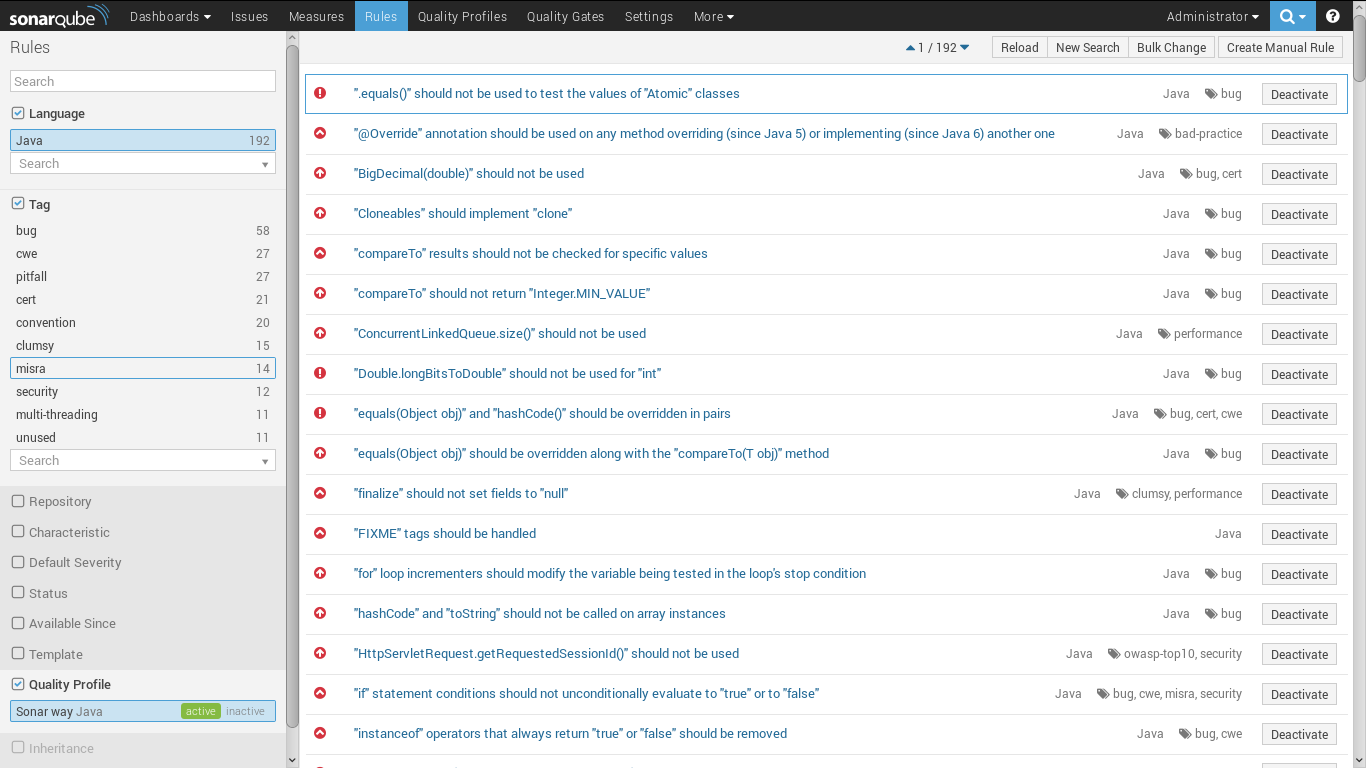
\includegraphics[scale=0.3]{img/sonarqube}
		\caption{Le paramétrage des règles du profil \emph{Sonar Way (Java)}}
		\label{fig:Sonarqube}
	\end{center}
\end{figure}

\section{Jenkins}
\subsection{Description}
\emph{Jenkins} est un serveur d'automatisation de compilation. Cet outil permet d'automatiser des compilations, des tests et le déploiement d'une application. De plus il est personnalisable avec des centaines de plugins.
\begin{figure}
	\begin{center}
		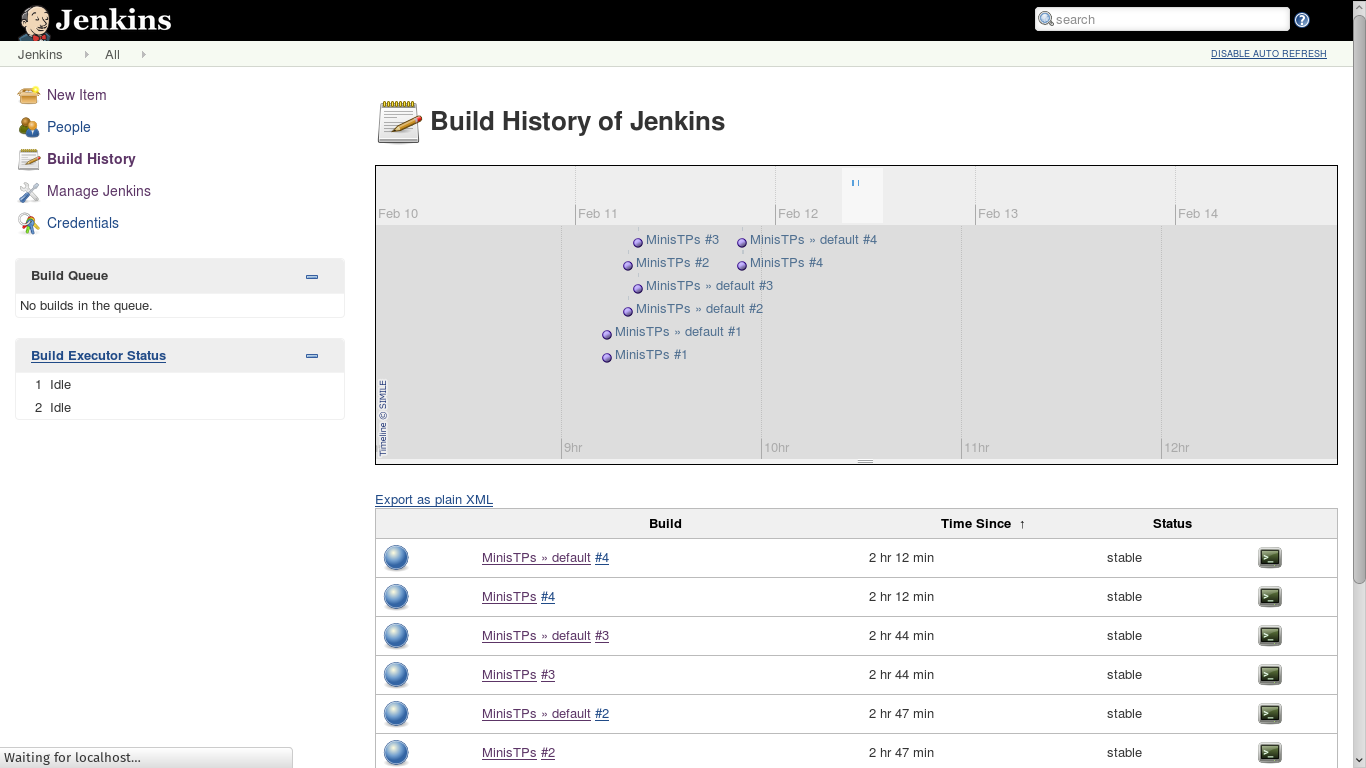
\includegraphics[scale=0.3]{img/jenkins}
		\caption{L'historique des builds de \emph{Jenkins}}
		\label{fig:Jenkins}
	\end{center}
\end{figure}
\subsection{Utilisation}
Ce TP nous a permis d'automatiser les builds d'un git distant. Dans notre cas, il s'agit du dépot disponible à l'adresse \url{https://github.com/AmarOk1412/MinisTPS8}. Ce dépot contenant plusieurs matières, nous avons créé un projet de type Multi-configurations et dans la partie \emph{Build}, nous avons ajouté un appel à un script shell contenant~:
\begin{minted}{bash}
	sh -c 'cd AL/TP1 && mvn clean package install'
\end{minted}
Bien sûr, ce script peut-être complété pour compiler tous les TPs et effectuer tous les tests.\\
Nous avons ensuite paramétré le \emph{pom.xml} de \emph{Maven} afin d'avoir un package propre en sortie de compilation. L'archive générée par la compilation automatisée est disponible dans le workspace (tout comme la sortie de la console, ce qui peut-être utile en cas de bug).
\subsection{Pourquoi l'utiliser ?}
Les outils d'intégration continue sont utiles car ils permettent de~:
\begin{itemize}
	\item Savoir quel commit a apporté un bug (automatisation des tests) et permet de savoir si quelque chose c'est mal déroulé sur une plateforme ce qui permet de prévenir les développeurs (mail) et de régler le problème rapidement.
	\item Pouvoir automatiser le déploiement de l'application sans suivi (et paramétrer des cycles de déploiement (par exemple tous les jours pour une version alpha, toutes les semaines pour une béta et tous les mois pour une version stable)).
\end{itemize}
D'autres outils existent comme \emph{Travis} qui est aussi utilisé sur le dépot (\url{https://travis-ci.org/AmarOk1412/MinisTPS8}).
\begin{figure}
	\begin{center}
		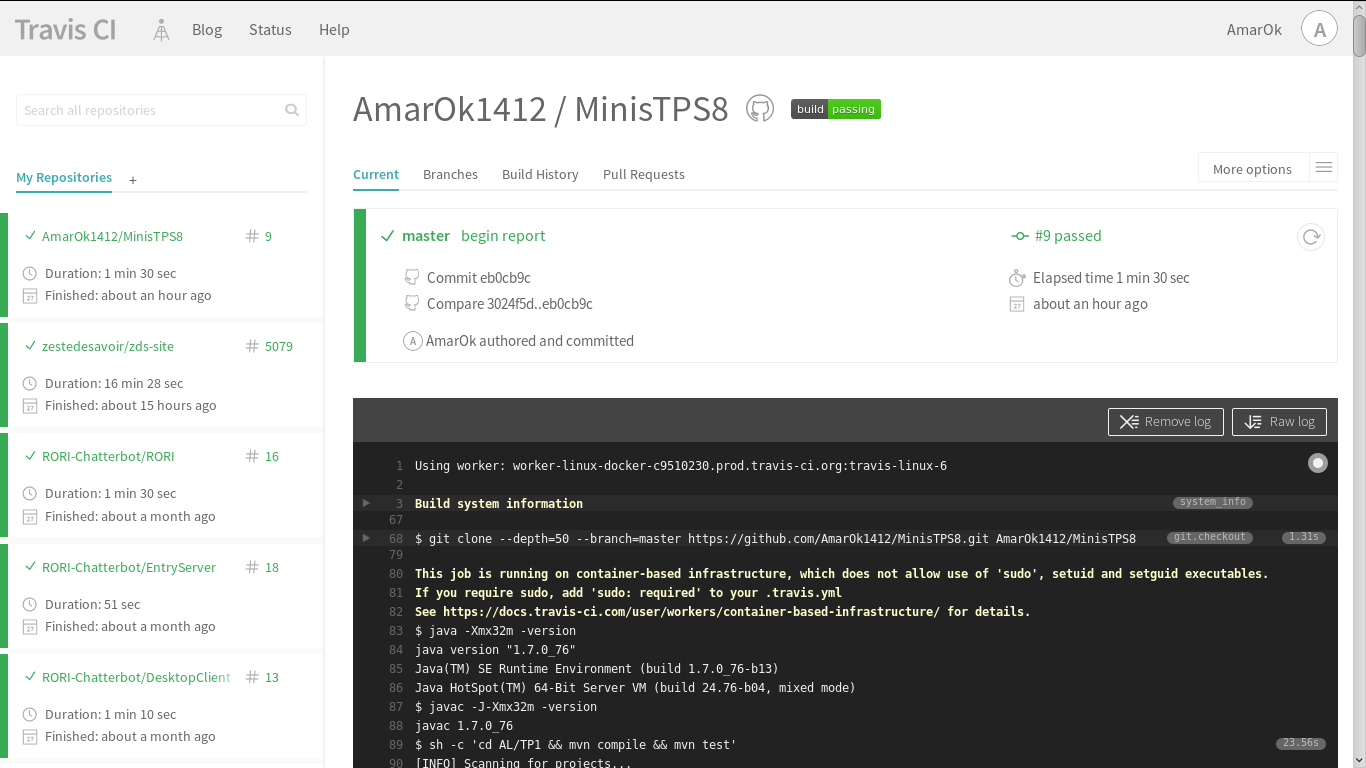
\includegraphics[scale=0.3]{img/travis}
		\caption{L'outil \emph{Travis-CI} sur le dépot du projet}
		\label{fig:Travis}
	\end{center}
\end{figure}
\end{document}
